\label{problemstatement}

\begin{table*}[!t]
\centering
\caption{Specific FM Approaches to Different NFV Layers}
\label{tbl:layers}
	\begin{tabular}{c|p{3cm}|p{5cm}}
		\hline
		\textbf{Layer} & \textbf{Typical HA Approaches} & \textbf{Example}\\
		\hline
		\hline
		Physical	&	Heartbeat, Fencing, Hot/Cold Standby, Reliable Messaging Bus &
LinuxHA Project, Pacemaker, cman \\
		Hypervisor & Virtual Resource Monitoring, Live Migration & VMWare HA, HA-Lizard \\
		Virtual Network Functions & Application-specific FM methods & vendor
specific application \\
		Virtual Services & Traditional Network Service OSS/BSS & SNMP or other
vendor specific methods to manage faults of virtual devices \\
\hline
	\end{tabular}
\end{table*} 
 
The central challenge in the cross-layer fault management lays in the coordination
of various FM appraoches from different layers involved in the NFV architecture
and, frequently, also within individual layers. We classify those problem in
\emph{vertical} and \emph{horizontal} dimensions. In this section, we analyze
research problems in details accrodingly to the above mentioned dimensions,
then we provide a scenario that clarify an uncoordinated FM will aggreviate the
holistic system when failures impact. 

\subsection{Problems of Vertical Integration of FM Approaches} 

Typically each layer of NFV architecture possesses its own specific FM
approaches to ensure the services offered on this particular layer as we
illustrate in the Table~\ref{tbl:layers}. There is hardly any information
exchanged between layers regarding FM and let alone the coordination of
separated layers, let alone the coordinations among them. We argue that such a
separate approach does not meet requirements of a high efficient overall FM
system. Failing to do so will introduce various sorts of inconsistent problems
in terms of false positives in failure detections, inconsistent fault recovery
actions, which will only aggravate the holistic fault management process in general.

\subsubsection{Virtualization and Physical Layers}

Virtualization enables physical resources to be shared among multiple virtual
instances in terms of computing, networking and storage. While there are
different forms of resource virtualization, e.g. server, network, application
etc., different approaches have been applied to manage the virtual instances
which mostly concentrate on the efficient control of physical resources.
Features such as tracking of dependencies between virtual resources and their
physical mappings from the service point of view is still missing piece. Such kind
of dependency tracking is essential for the reliability both from top-down and
bottom-up perspective. When fault impacts virtualized resources, FM should
tracking down the associated physical resources so that new resources could be
employed to mitigate faults and vice versa. This requires precise mappings
between layers since there could be one-to-many (aggregation) or many-to-one
(sharing) relationships between virtualized and physical resources as shown in
Fig.\ref{fig:mapping}.  
 
\begin{figure}[ht]
	\centering
	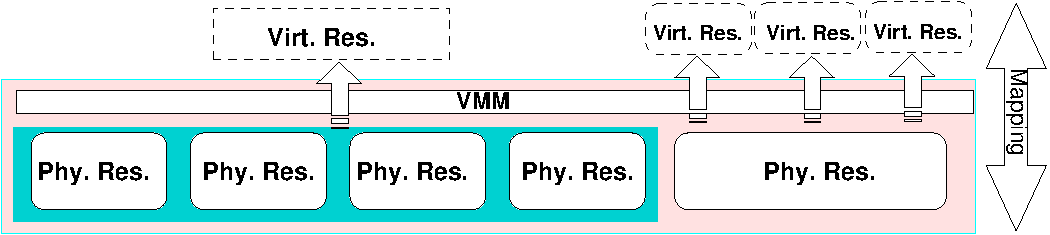
\includegraphics[scale=0.52]{fig/mapping.pdf}
	\caption{Mapping of virtual and physical resources}
	\label{fig:mapping}
\end{figure}

As suggested in the Table~\ref{tbl:layers}, on the physical layer, FM approaches
such as heartbeats and fencing are usually applied to ensure the high
availability of clusters. On the virtualization layer, monitoring mechanisms
frequently focus on the health of virtual resources, there is hardly any
communication between separate approaches. Configuration as such can introduce
inconsistency not only during the FM operations, since each layer makes
decisions based on its own observations of current states of its own, e.g.  in a
one-to-many configuration, heartbeat mechanism managing HA of physical clusters
decides to apply Totem single-ring ordering and membership
protocol~\cite{amir1995totem} (e.g. Corosync) to shutdown and replace a node
which does not respond to heartbeat, however in the same moment, management of
virtual resources also detects the service degradation, but decides to migrate
the complete virtual element onto other set of working nodes in their resource
pool. This scenario leads to extra overhead for he unnecessary operations due to
lack of communication between layers and thus inconsistency in the fault
management actions derived.
 
\subsubsection{NFVI and NFV Layers}

Same mapping and consistency problems could affect NFVI and NFV layers as well,
where NFVIs are virtualized teleco services elements and NFV is teleco services
chained together by an orchestration function using service elements. Virtualized
infrastructure is provisioned based on virtual resources prepared by hypervisors
and other different means of virtualization, e.g. storage and network
virtualization techniques. On NFVI layer, virtual resources are combined with
specific functionalities such as vRouters, vEPC, vFirewall etc. as shown on the
top layer in Fig.~\ref{fig:arch}. An orchestration functions   


\subsection{Problems of Horizontal Integration of FM Approaches}

\subsubsection{Coordinations between Distributed Clusters}

\subsubsection{Multi-Orchestrator Collaboration}
